\documentclass[11pt]{article}

%  Packages
\usepackage[
   paperheight = 11.0in,
   paperwidth = 8.5in,
   tmargin = 1in,
   bmargin = 1in,
   lmargin = 1in,
   rmargin = 1in,
   footskip = 0.50in] {geometry}
\usepackage{float} %  better floats
\usepackage{enumitem} %  better enumerations
\usepackage{amsmath} %  better math layout
\usepackage{bm} %  bold math (must be after amsmath)
\usepackage{cancel} %  strick-through in equations
\usepackage{tikz} %  drawing
\usepackage{color} %  custom colors
\usepackage[breakable, theorems, skins]{tcolorbox}
\usepackage{listings, upquote} %  "\lstinline{ }" for inline code
\usepackage[
   colorlinks = true,
   linkcolor = blue,
   urlcolor = blue,
   hypertexnames = false]{hyperref}

%  Parameters
\setlength\emergencystretch{\hsize}
\setlength{\arraycolsep}{2pt} %  matrix column spacing
\renewcommand{\arraystretch}{1.4} %  matrix row spacing
\newtcolorbox{example}{
   breakable,
   colframe = shade,
   colback = shade,
   before skip = 10pt,
   after skip = 10pt}

%  Custom macros
\renewcommand{\vec}[1]     {\bm{#1}} %  vectors
\newcommand{\mat}[1]       {\bm{#1}} %  matrices
\renewcommand{\exp}[1]     {\mathrm{e}^{#1}}
\renewcommand{\cos}[2][]   {\mathrm{cos}^{#1}\!\left( {#2} \right)}
\renewcommand{\sin}[2][]   {\mathrm{sin}^{#1}\!\left( {#2} \right)}
\renewcommand{\tan}[2][]   {\mathrm{tan}^{#1}\!\left( {#2} \right)}
\newcommand{\acos}[1]      {\mathrm{acos}\!\left( {#1} \right)}
\newcommand{\asin}[1]      {\mathrm{asin}\!\left( {#1} \right)}
\newcommand{\atan}[1]      {\mathrm{atan}\!\left( {#1} \right)}
\renewcommand{\log}[2][]   {\mathrm{log}_{#1}\!\left( {#2} \right)}
\newcommand{\EE}[2]        {{#1}\textsc{e}\mathrm{#2}}

\definecolor{red}          {rgb}{1.00,0.00,0.00}
\definecolor{orange}       {rgb}{1.00,0.50,0.00}
\definecolor{yellow}       {rgb}{1.00,0.83,0.00}
\definecolor{green}        {rgb}{0.00,0.60,0.00}
\definecolor{cyan}         {rgb}{0.00,0.90,0.90}
\definecolor{blue}         {rgb}{0.00,0.50,1.00}
\definecolor{purple}       {rgb}{0.50,0.00,1.00}
\definecolor{magenta}      {rgb}{1.00,0.00,1.00}
\definecolor{gray}         {rgb}{0.50,0.50,0.50}
\definecolor{shade}        {rgb}{0.95,0.95,0.95}

\lstdefinestyle{lstMat} {
   language = matlab,
   backgroundcolor = {},
   breakatwhitespace = true,
   breaklines = true,
   showstringspaces = false,
   basicstyle = %
   \lst@ifdisplaystyle\footnotesize\fi
   \ttfamily, %  48 chars in 3.5 in
   commentstyle = \color{green},
   stringstyle = \color{magenta},
   tabsize = 3,
   upquote = true}
\lstset{style = lstMat}

\title{Lab 1 Report}
\author{Rick Yuan}

\begin{document}

\maketitle

Step 1: system dynamics equations
The system dynamics for the two states
\begin{equation}
	\dot{x}_1=x_2
\end{equation}
\begin{equation}
	\dot{x}_2=-G*m_1*m_2/r^2 + F_\mathrm{thrust}
\end{equation}

Step 2: force of gravity at surface
\begin{equation}
	G_0=-G*m_1*m_2/r^2=-2.9995*10^3
\end{equation}

Step 3: derivative of gravity
\begin{equation}
	\delta F_g/\delta x=2*G*m_1*m_2/(r_a +x)^2
\end{equation}
At X = 0:
\begin{equation}
	\delta F_g/\delta x=2*G*m_1*m_2/(r_a )^2 = 5.9990
\end{equation}

Step 4: linear model of gravity
Linear model of gravity
\begin{equation}
	F_\mathrm{Glinear} = -2.9995*10^3 + 5.9990*x_1
\end{equation}
\\
2.022\% error at x=80\\
13.60\% error at x=200\\
100\% error at x=500\\

Step 5: linear state space system
\begin{equation}
\begin{array}{l}
\dot{X} = FX + BU\\
Y = HX\\
F = 
\begin{pmatrix}
0 & 1\\
0.006 & 0
\end{pmatrix}\\
B = 
\begin{pmatrix}
0 & 0\\
0.001 & 0.001\\
\end{pmatrix}\\
H = 
\begin{pmatrix}
1 \\
0\\
\end{pmatrix}\\
\end{array}
\end{equation}
Step 6: discretized state space system at 0.1 seconds
\begin{equation}
\begin{array}{l}
\Phi=
\begin{pmatrix}
1 & 0.1\\
0.0006 & 1\\
\end{pmatrix}\\ 
B = 10^-3*
\begin{pmatrix}
0.005 & 0.005\\
0.1 & 0.1\\
\end{pmatrix}\\
\end{array}
\end{equation}
Step 7: Matlab code to compute next state

%\item To add Matlab code, upload your file and include it here:
        \lstinputlisting{SpaceX_student_function.m}
        %\newpage

Step 8: successful landing
\begin{figure}[H]
            \centering
            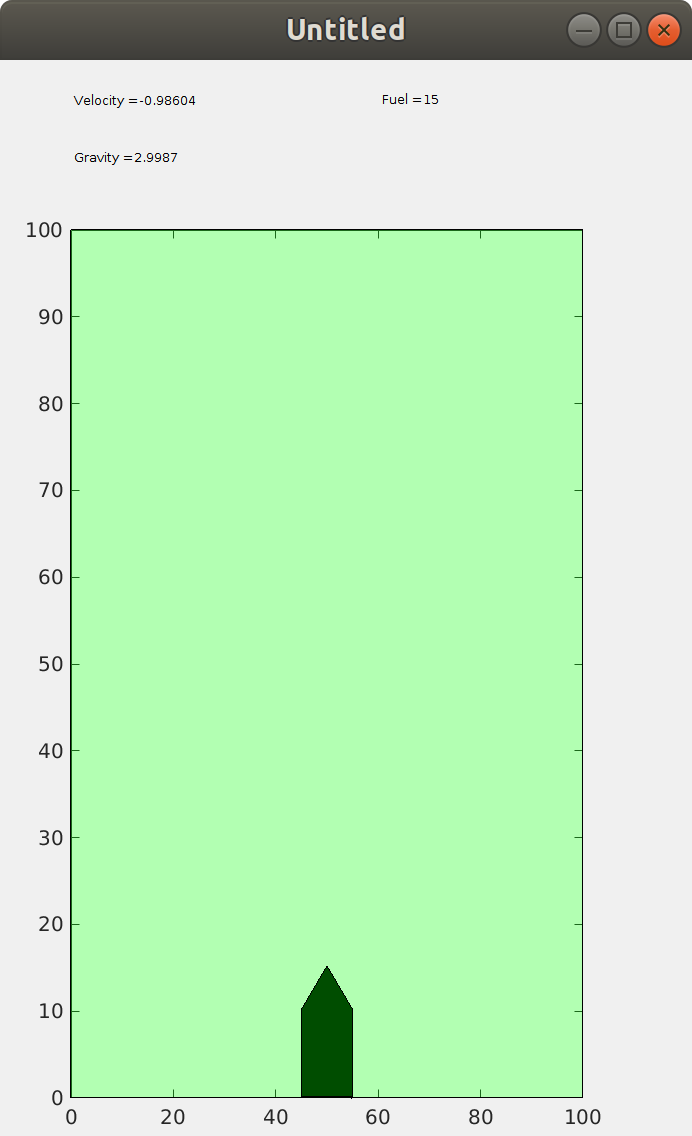
\includegraphics[width=15cm]{winning landing.png}
\end{figure}
Step 9: 
\lstinputlisting{SpaceX_student_script.m}

Step 10: plotting
\begin{figure}[H]
            \centering
            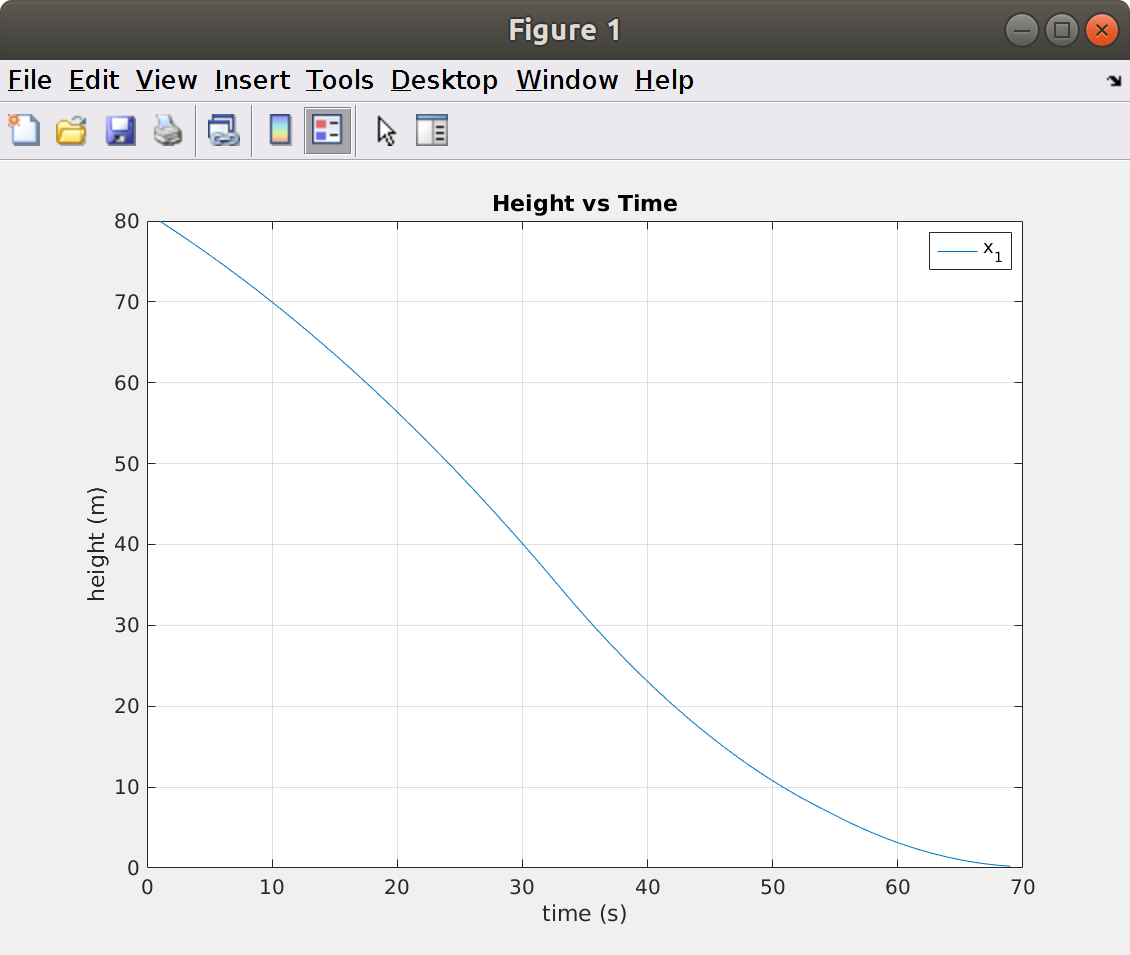
\includegraphics[width=15cm]{fig1.png}
\end{figure}
\begin{figure}[H]
            \centering
            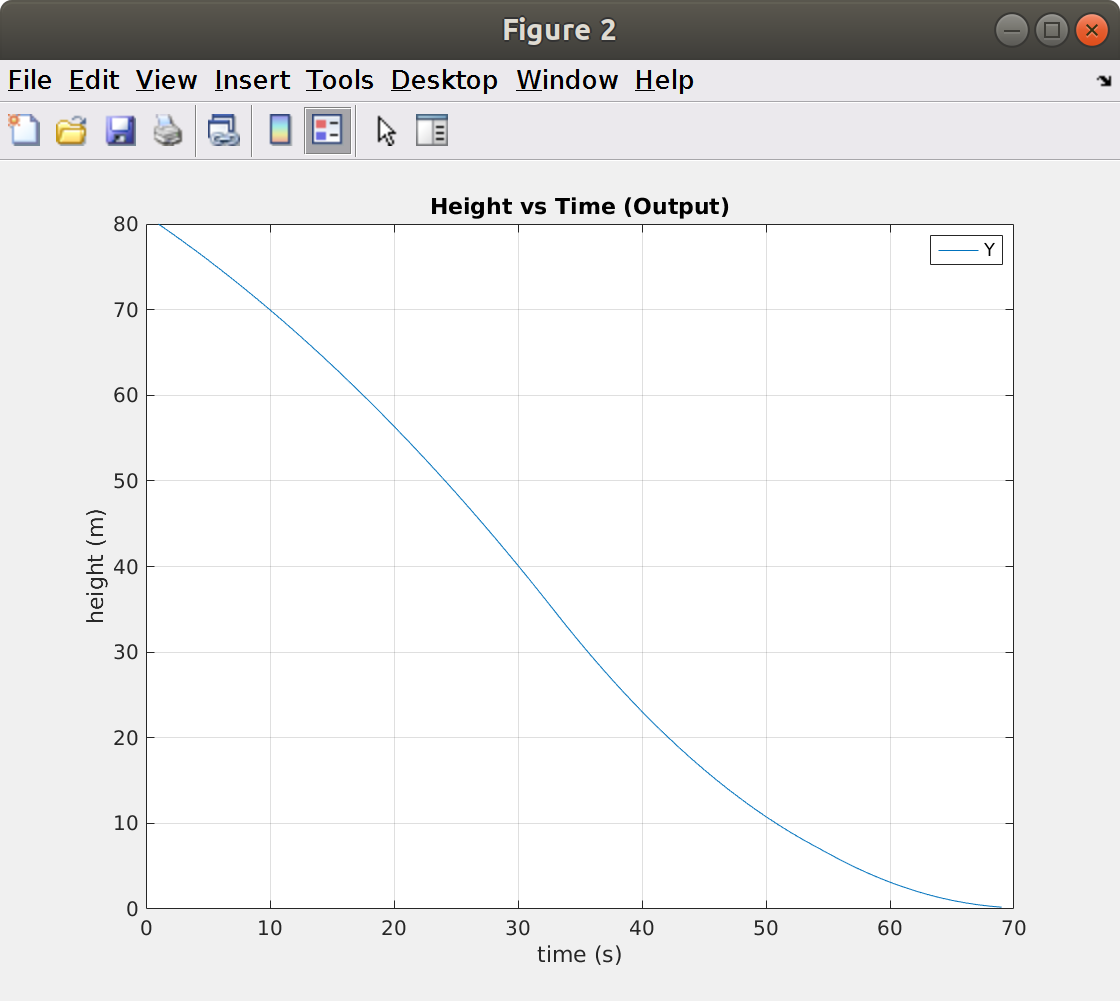
\includegraphics[width=15cm]{fig2.png}
\end{figure}
\begin{figure}[H]
            \centering
            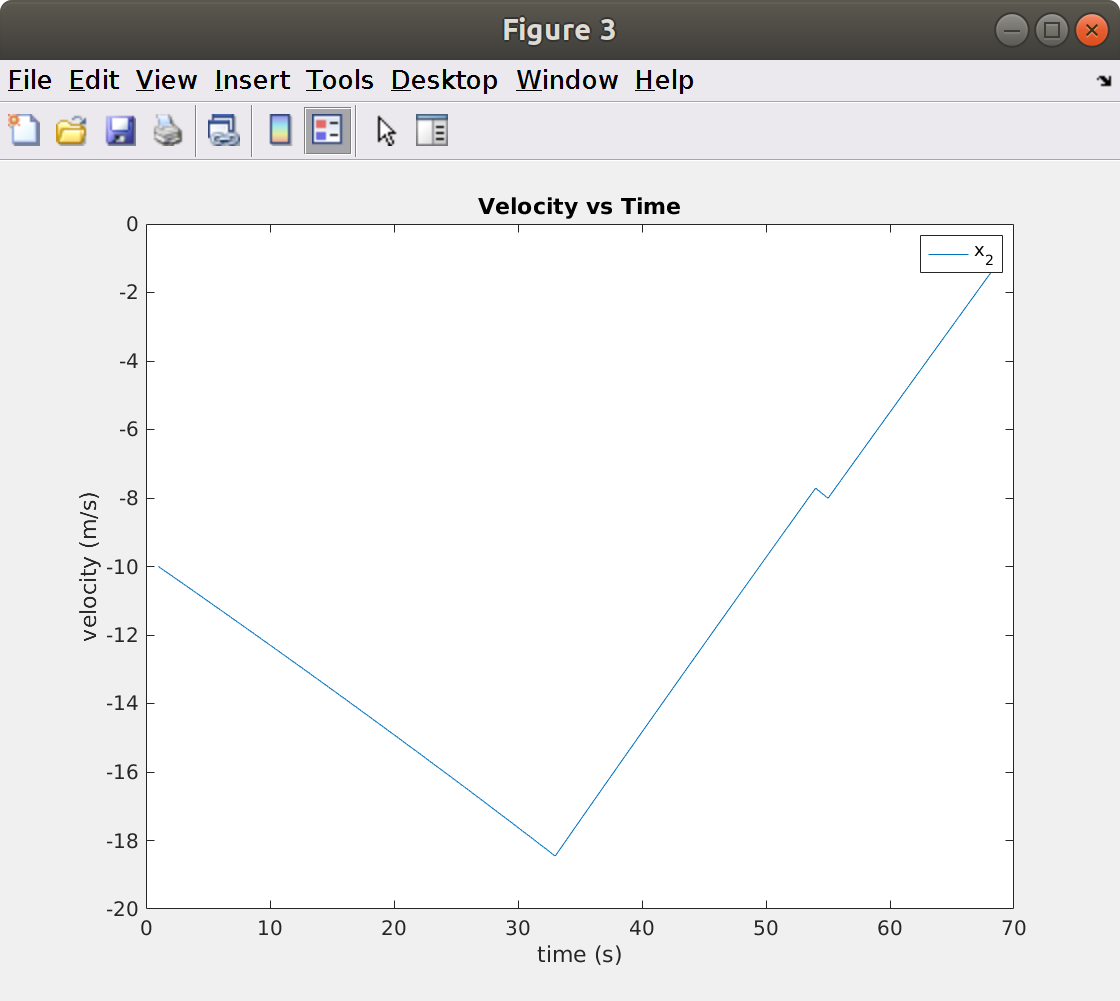
\includegraphics[width=15cm]{fig3.png}
\end{figure}


\begin{lstlisting}[style=lstMat]
The output will always be equal to the state x_1 because it is simply multiplied by 1 to get the output.

Step 11:
Rerunning the script with the discrete B matrix approximated as B*0.1, the new final velocity of the rocket is -0.9800 m/s. This represents a 0.6 percent error in the final velocity 
\end{lstlisting}
Other Matlab Code:\\
Project1.m
	\lstinputlisting{Project1.m}


\end{document}

